\documentclass{beamer}
\usepackage{polski}
\usepackage[utf8x]{inputenc}
\usepackage{default,longtable}
\title{Wizualizacja ontologii zapisanych w języku OWL}
\author{Piotr Kunowski}
\mode<presentation>
{
\usetheme{Warsaw}
}
\begin{document}
\def\protege{Prot\'{e}g\'{e}}
\begin{frame}
  \titlepage
\end{frame}

\section{Motto}
\begin{frame}
\begin{block}{motto} 

"Wiedza nie wystarczy, musimy ją stosować. \\
Wola nie wystarczy, musimy działać."
\begin{flushright}
J. W. Goethe
\end{flushright}
\end{block}
 

\end{frame}


\section{Definicja problemu}

\subsection{Cel pracy}

\begin{frame}
  \frametitle{Cel pracy}
  \begin{block}{Cel}
	Celem pracy jest zaprojektowanie oraz zaimplementowanie biblioteki umożliwiającej wizualizację w przejrzysty 
sposób dowolnie złożonej ontologii zdefiniowanej w języku OWL oraz przechowywanej w postaci obiektów OWL API
  \end{block}
\end{frame}

\section{SOVA}
\begin{frame}
	\frametitle{SOVA}
	 \begin{block}{SOVA}
		Simple Ontology Visualization API
	\end{block} 
\end{frame}

\begin{frame}
	\frametitle{Wizualizacja elementów OWL}
	
\begin{longtable}{lp{7cm}} 

  Thing &
 \scalebox{0.30}{
\includegraphics{./elementyGraficzne/drobne/thing.png}}
 % class.png: 194x86 pixel, 90dpi, 5.48x2.43 cm, bb=0 0 155 69
 \\ 

  Nothing &
 \scalebox{0.30}{
\includegraphics{./elementyGraficzne/drobne/nothing.png}}
 % class.png: 194x86 pixel, 90dpi, 5.48x2.43 cm, bb=0 0 155 69
 \\ 

  Class &
 \scalebox{0.30}{
\includegraphics{./elementyGraficzne/drobne/class.png}}
 % class.png: 194x86 pixel, 90dpi, 5.48x2.43 cm, bb=0 0 155 69
 \\ 

  Individual &
 \scalebox{0.30}{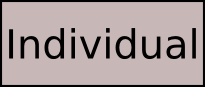
\includegraphics{./elementyGraficzne/drobne/individual.png}}
 % class.png: 194x86 pixel, 90dpi, 5.48x2.43 cm, bb=0 0 155 69
 \\ 

  Property &
 \scalebox{0.30}{
\includegraphics{./elementyGraficzne/drobne/property.png}}
 % class.png: 194x86 pixel, 90dpi, 5.48x2.43 cm, bb=0 0 155 69
 \\ 

  Datatype &
 \scalebox{0.30}{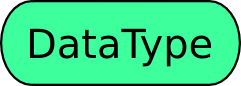
\includegraphics{./elementyGraficzne/drobne/datatype.png}}
 % class.png: 194x86 pixel, 90dpi, 5.48x2.43 cm, bb=0 0 155 69
 \\ 

  Anonymous Class &
 \scalebox{0.30}{
\includegraphics{./elementyGraficzne/drobne/anonymousClass.png}}
 % class.png: 194x86 pixel, 90dpi, 5.48x2.43 cm, bb=0 0 155 69
 \\ 

  Subclass &
 \scalebox{0.30}{
\includegraphics{./elementyGraficzne/drobne/subclass.png}}
 % class.png: 194x86 pixel, 90dpi, 5.48x2.43 cm, bb=0 0 155 69
 \\ 


\end{longtable}
\end{frame}


\begin{frame}
	\frametitle{Wizualizacja elementów OWL}
	
\begin{longtable}{lp{7cm}} 
 instanceOf &
 \scalebox{0.30}{
\includegraphics{./elementyGraficzne/drobne/instanceOf.png}} \newline
 \scalebox{0.30}{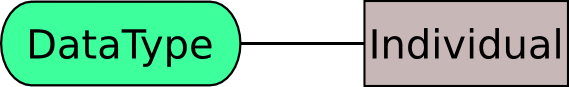
\includegraphics{./elementyGraficzne/drobne/instanceOfDatatype.png}}
 % class.png: 194x86 pixel, 90dpi, 5.48x2.43 cm, bb=0 0 155 69
 \\  

equivalentClass &
 \scalebox{0.30}{
\includegraphics{./elementyGraficzne/drobne/equivalentClass.png}}
 % class.png: 194x86 pixel, 90dpi, 5.48x2.43 cm, bb=0 0 155 69
 \\ 

  disjointWith &
 \scalebox{0.30}{
\includegraphics{./elementyGraficzne/drobne/disjointWith.png}}
 % clas.png: 194x86 pixel, 90dpi, 5.48x2.43 cm, bb=0 0 155 69
 \\ 

  differentFrom / allDifferent &
 \scalebox{0.30}{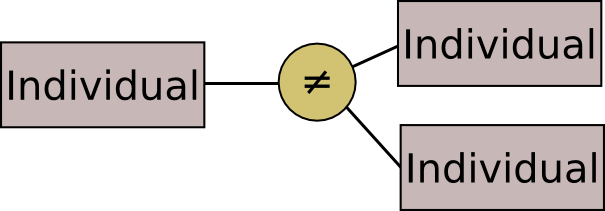
\includegraphics{./elementyGraficzne/drobne/allDifferent.png}}
 % class.png: 194x86 pixel, 90dpi, 5.48x2.43 cm, bb=0 0 155 69
 \\ 

  sameAs &
 \scalebox{0.30}{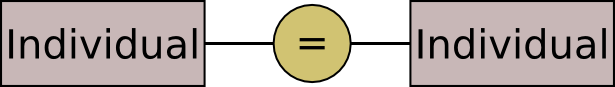
\includegraphics{./elementyGraficzne/drobne/sameAs.png}}
 % class.png: 194x86 pixel, 90dpi, 5.48x2.43 cm, bb=0 0 155 69
 \\ 

\end{longtable}
\end{frame}


\begin{frame}
	\frametitle{Wizualizacja elementów OWL}
	
\begin{longtable}{lp{7cm}} 
 

  oneOf &
 \scalebox{0.30}{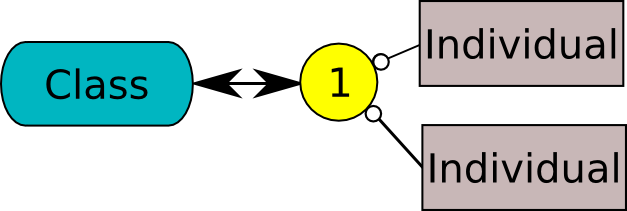
\includegraphics{./elementyGraficzne/drobne/oneOf.png}}
 % class.png: 194x86 pixel, 90dpi, 5.48x2.43 cm, bb=0 0 155 69
 \\ 

  unionOf &
 \scalebox{0.30}{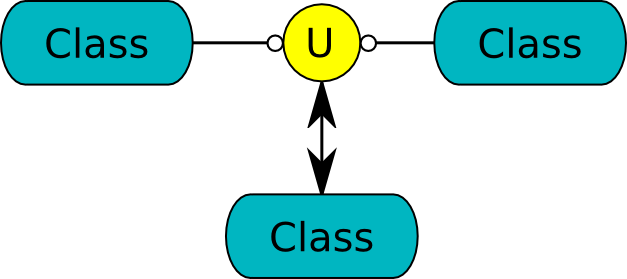
\includegraphics{./elementyGraficzne/drobne/unionOf.png}}
 % class.png: 194x86 pixel, 90dpi, 5.48x2.43 cm, bb=0 0 155 69
 \\ 

  intersectionOf &
 \scalebox{0.30}{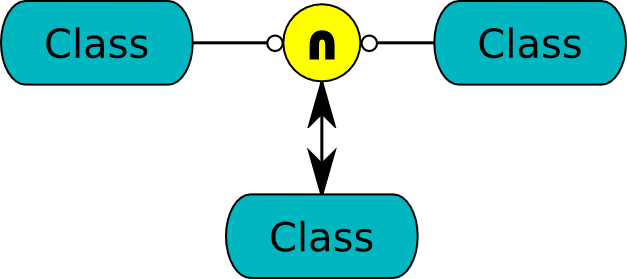
\includegraphics{./elementyGraficzne/drobne/intersectionOf.png}}
 % class.png: 194x86 pixel, 90dpi, 5.48x2.43 cm, bb=0 0 155 69
 \\ 


\end{longtable}
\end{frame}


\begin{frame}
	\frametitle{Wizualizacja elementów OWL}
	
\begin{longtable}{lp{7cm}} 
 

  complementOf &
 \scalebox{0.30}{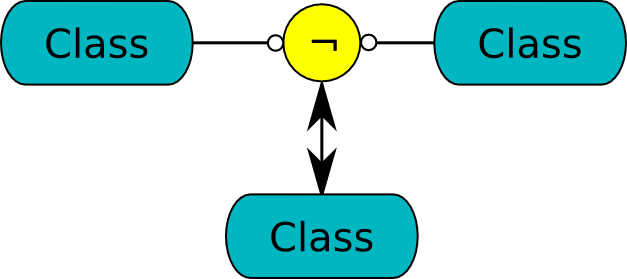
\includegraphics{./elementyGraficzne/drobne/complementOf.png}}
 % class.png: 194x86 pixel, 90dpi, 5.48x2.43 cm, bb=0 0 155 69
 \\ 

  subProperty &
 \scalebox{0.30}{
\includegraphics{./elementyGraficzne/drobne/subProperty.png}}
 % class.png: 194x86 pixel, 90dpi, 5.48x2.43 cm, bb=0 0 155 69
 \\ 

  inverseOf (property) &
 \scalebox{0.30}{
\includegraphics{./elementyGraficzne/drobne/inverseOf.png}} \newline
\scalebox{0.30}{
\includegraphics{./elementyGraficzne/drobne/inverseOfProperty.png}}
 % class.png: 194x86 pixel, 90dpi, 5.48x2.43 cm, bb=0 0 155 69
 \\ 

  equivalentProperty &
 \scalebox{0.30}{
\includegraphics{./elementyGraficzne/drobne/equivalentProperty.png}}
 % class.png: 194x86 pixel, 90dpi, 5.48x2.43 cm, bb=0 0 155 69
 \\ 

\end{longtable}
\end{frame}




\begin{frame}
	\frametitle{Wizualizacja elementów OWL}
	
\begin{longtable}{lp{7cm}} 
 
  functionalProperty &
 \scalebox{0.30}{
\includegraphics{./elementyGraficzne/drobne/functionalProperty.png}}
 % class.png: 194x86 pixel, 90dpi, 5.48x2.43 cm, bb=0 0 155 69
 \\ 

  inverseFunctionalProperty &
 \scalebox{0.30}{
\includegraphics{./elementyGraficzne/drobne/inverseFunctionalProperty.png}}
 % class.png: 194x86 pixel, 90dpi, 5.48x2.43 cm, bb=0 0 155 69
 \\ 

  symmetricProperty &
 \scalebox{0.30}{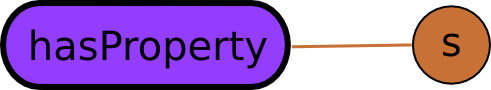
\includegraphics{./elementyGraficzne/drobne/symmetricProperty.png}}
 % class.png: 194x86 pixel, 90dpi, 5.48x2.43 cm, bb=0 0 155 69
 \\ 

  transitiveProperty &
 \scalebox{0.30}{
\includegraphics{./elementyGraficzne/drobne/transitiveProperty.png}}
 % class.png: 194x86 pixel, 90dpi, 5.48x2.43 cm, bb=0 0 155 69
 \\ 

  hasProperty &
 \scalebox{0.25}{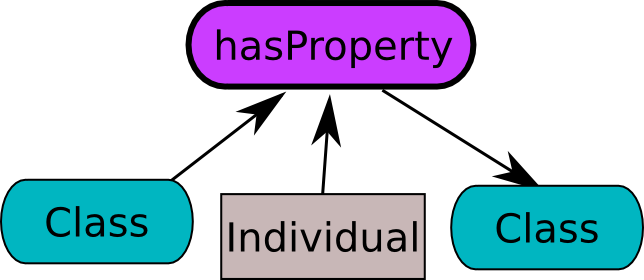
\includegraphics{./elementyGraficzne/drobne/hasProperty.png}}
 % class.png: 194x86 pixel, 90dpi, 5.48x2.43 cm, bb=0 0 155 69
 \\ 

  domain &
 \scalebox{0.25}{
\includegraphics{./elementyGraficzne/drobne/domain.png}}
 % class.png: 194x86 pixel, 90dpi, 5.48x2.43 cm, bb=0 0 155 69
 \\ 

  range &
 \scalebox{0.25}{
\includegraphics{./elementyGraficzne/drobne/range.png}}
 % class.png: 194x86 pixel, 90dpi, 5.48x2.43 cm, bb=0 0 155 69
 \\ 



\end{longtable}
\end{frame}


\begin{frame}
	\frametitle{Wizualizacja elementów OWL}
\begin{longtable}{lp{7cm}} 


  allValuesFrom &
 \scalebox{0.25}{
\includegraphics{./elementyGraficzne/drobne/allValuesFrom.png}}
 % class.png: 194x86 pixel, 90dpi, 5.48x2.43 cm, bb=0 0 155 69
 \\ 

  someValuesFrom &
 \scalebox{0.25}{
\includegraphics{./elementyGraficzne/drobne/someValuesFrom.png}}
 % class.png: 194x86 pixel, 90dpi, 5.48x2.43 cm, bb=0 0 155 69
 \\ 

  minCardinality / maxCardinality &
 \scalebox{0.30}{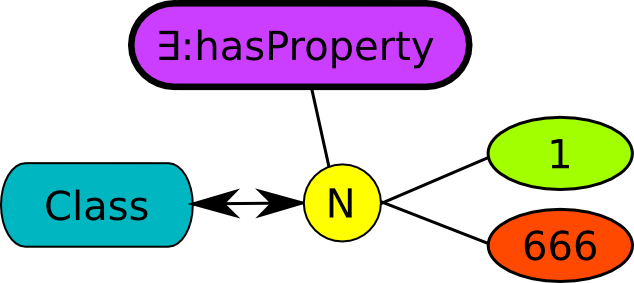
\includegraphics{./elementyGraficzne/drobne/cardinalityminmax.png}}
 % class.png: 194x86 pixel, 90dpi, 5.48x2.43 cm, bb=0 0 155 69
 \\ 

  cardinality &
 \scalebox{0.30}{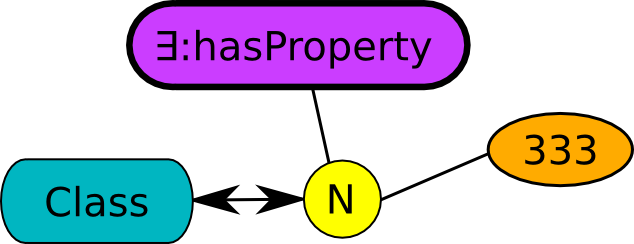
\includegraphics{./elementyGraficzne/drobne/cardinality.png}}
 % class.png: 194x86 pixel, 90dpi, 5.48x2.43 cm, bb=0 0 155 69
 \\ 


\end{longtable}
\end{frame}

\begin{frame}
 \frametitle{}
Zaimplementowane moduły: 
\begin{itemize}
  \item Biblioteka do wizualizacji - SOVA
  \item Plugin do \protege
  \item Moduł wizualizacji w systemie OCS
\end{itemize}

\end{frame}

\begin{frame}
 \frametitle{Komponenty programowe}
  \begin{itemize}
   \item{\bf Prefuse }

Biblioteka graficzna do wizualizacji grafów w języku Java

\item{\bf OWLAPI}

      Biblioteka do przetwarzania ontologii zapisanych w języku OWL. Napisana w języku Java.

  \end{itemize}

\end{frame}

\begin{frame}
 \frametitle{Biblioteka SOVA}
\begin{center}
 \scalebox{0.20}{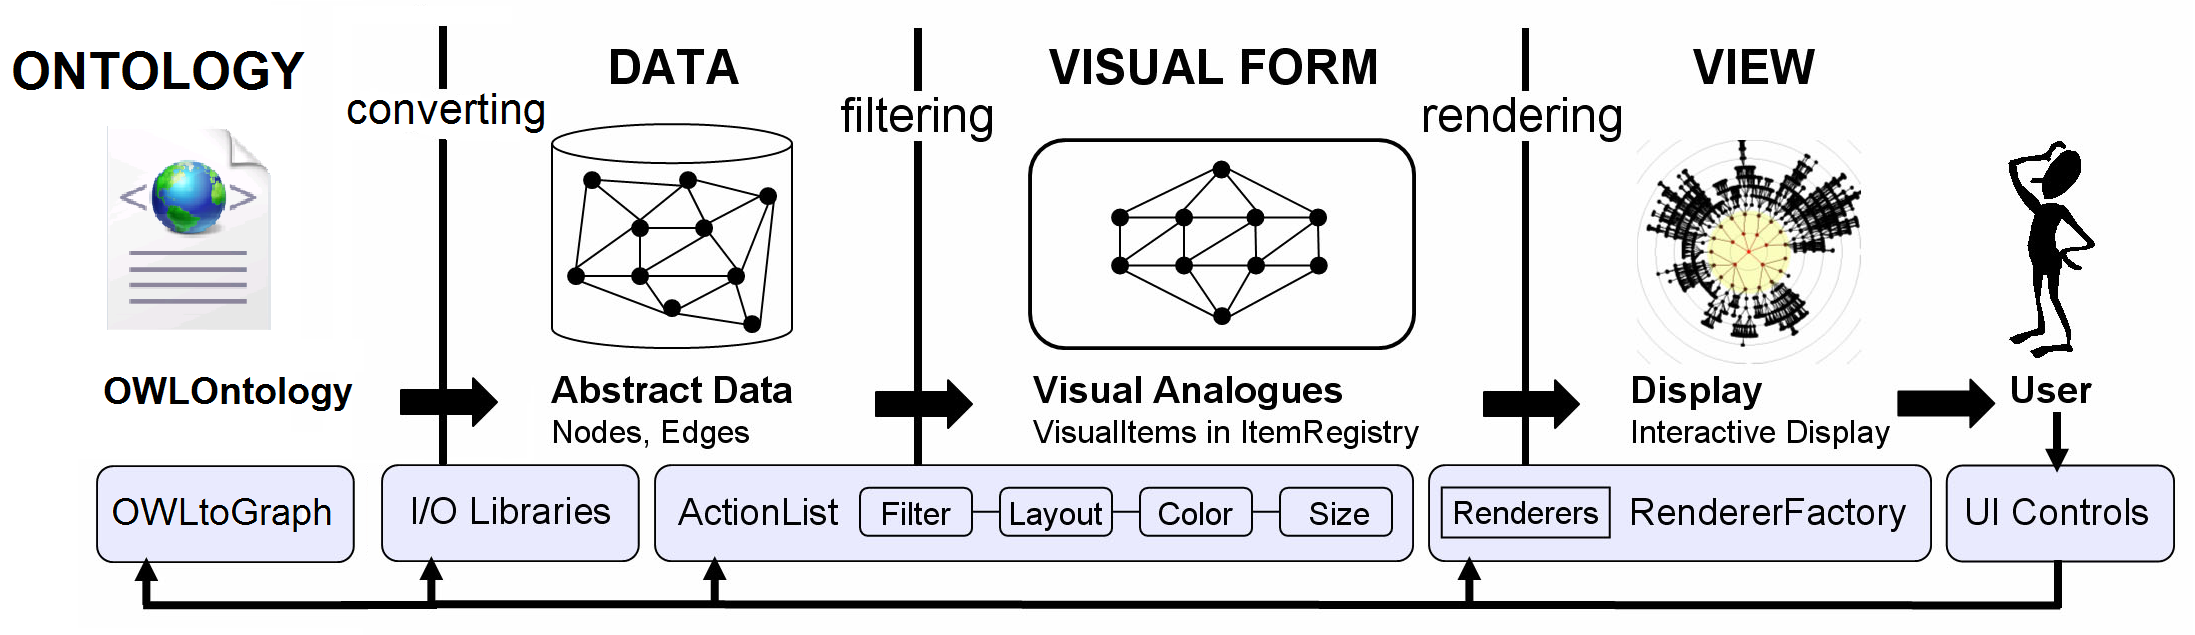
\includegraphics{./elementyGraficzne/prefuse.png}} 
\end{center}

\end{frame}

\begin{frame}
 \frametitle{Sposoby wizualizacji}
\begin{itemize}
 \item wizualizacja prosta
  \begin{itemize}
   \item ForceDirectedLayout
  \item RadialTreeLayout
  \end{itemize}

\item wizualizacja wywnioskowanej hierarchii klas i bytów
\end{itemize}

\end{frame}
\begin{frame}
 \frametitle{Filtry}
  W celu poprawienia przejrzystości wizualizacji wprowadzone zostały następujące filtry:
  \begin{itemize}
   \item filtr na elementy
   \item filtr na odległość od zaznaczonego elementu
  \end{itemize}

\end{frame}

\begin{frame}
 \frametitle{Problemy implementacyjne}

\begin{itemize}
  \item Słaba dokumentacja Prefuse
  \item Słaba dokumentacja OWLAPI 
\end{itemize}



\end{frame}


\begin{frame}
 \begin{center}
  {\bf Kiedy koniec?
\newline  Czyli podsumowanie stanu zaawansowania pracy magisterskiej.}
 \end{center}



\end{frame}


\end{document}
